% Author: Izaak Neutelings (June 2017)
\documentclass[border=3pt,tikz]{standalone}
\usepackage{tikz}
\tikzset{>=latex} % for LaTeX arrow head

\begin{document}

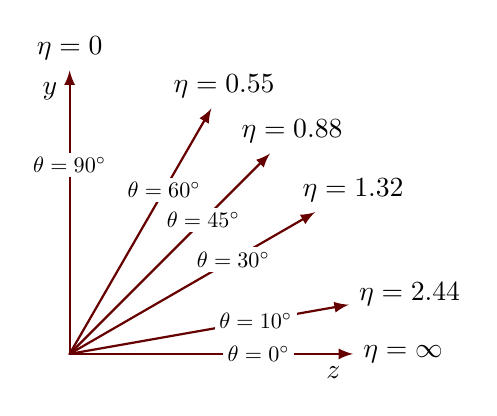
\begin{tikzpicture}[scale=3]
  \def\R{1.2} % radius/length of lines
  \node[scale=1,below left=1] at (0,\R) {$y$}; % y axis
  \node[scale=1,below left=1] at (\R,0) {$z$}; % z axis
  \foreach \t/\e in {90/0,60/0.55,45/0.88,30/1.32,10/2.44,0/\infty}{
    \draw[->,black!60!red,thick,line cap=round] % eta lines
      (0,0) -- (\t:\R) node[anchor=180+\t,black] {$\eta=\e$};
    \node[fill=white,scale=0.8,inner sep=2] at (\t:0.8) {$\theta=\t^\circ$};
  }
  %\draw[black!60!red,thick] (0,0.1*\R) |- (0.1*\R,0) ; % overlap in corner
\end{tikzpicture}

\end{document}